\documentclass[thesis.tex]{subfile}
\begin{document}
\chapter{Results} \label{Results}
\section{Control Group} \label{sec:Control Group}
First, we must verify that our localization system works well in Gazebo's noiseless environment. To do this, we examine the \gls{con_filter} state estimate error, specifically the horizontal distance and yaw error, for both a stationary robot and a randomly moving robot.

\subsection{Stationary Robot}

% Table created by stargazer v.5.2 by Marek Hlavac, Harvard University. E-mail: hlavac at fas.harvard.edu
% Date and time: Wed, Aug 10, 2016 - 04:38:08 PM
\begin{table}[h] \centering 
  \caption{Continuous Filter Estimate for one-stationary-noiseless-no-gps Experiment} 
  \label{tab:one_stationary_noiseless_no_gps_continuous_summary} 
\begin{tabular}{@{\extracolsep{5pt}}lccccc} 
\\[-1.8ex]\hline 
\hline \\[-1.8ex] 
Statistic & \multicolumn{1}{c}{N} & \multicolumn{1}{c}{Mean} & \multicolumn{1}{c}{St. Dev.} & \multicolumn{1}{c}{Min} & \multicolumn{1}{c}{Max} \\ 
\hline \\[-1.8ex] 
x\_position & 493 & 0.000 & 0.000 & $-$0 & 0 \\ 
y\_position & 493 & $-$0.000 & 0.000 & $-$0 & 0 \\ 
yaw & 493 & 0.000 & 0.000 & $-$0 & 0 \\ 
x\_variance & 493 & 1.541 & 0.846 & 0.081 & 3.002 \\ 
y\_variance & 493 & 1.541 & 0.846 & 0.081 & 3.002 \\ 
yaw\_variance & 493 & 1.847 & 1.014 & 0.097 & 3.599 \\ 
yaw\_error & 493 & 0.0002 & 0.0001 & 0.0001 & 0.0004 \\ 
x\_error & 493 & 0.0003 & 0.0001 & 0.00001 & 0.001 \\ 
y\_error & 493 & 0.00000004 & 0.00000003 & 0.000 & 0.0000001 \\ 
horizontal\_error & 493 & 0.0003 & 0.0001 & 0.00001 & 0.001 \\ 
\hline \\[-1.8ex] 
\end{tabular} 
\end{table} 


\begin{figure}
\centering
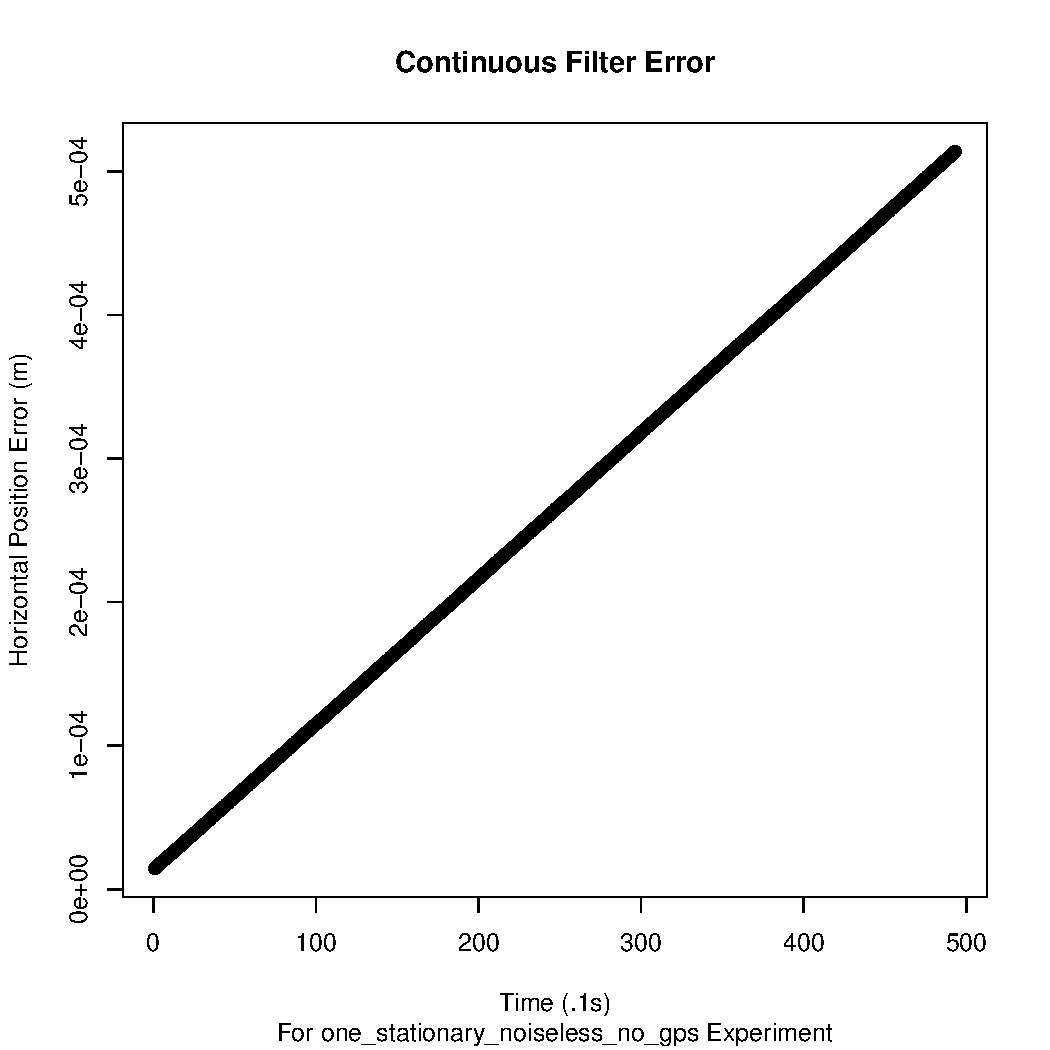
\includegraphics[width=\textwidth, keepaspectratio]{one_stationary_noiseless_no_gps_continuous_error}
\caption{Error of \gls{con_filter} of Stationary Robot with Noiseless Odometry Over Time}
\label{fig:one_stationary_noiseless_no_gps_continuous_error}
\end{figure}

For a stationary robot in a noiseless environment we can see in \autoref{tab:one_stationary_noiseless_no_gps_continuous_summary} and \autoref{fig:one_stationary_noiseless_no_gps_continuous_error} that the \gls{con_filter} tracks the Gazebo ground truth odometry almost perfectly. The maximum horizontal error is $2\times 10^{-6}$ m and the maximum yaw error is $4\times10^{-5}$ radians. These errors would be completely indistinguishable from perfect accuracy in the real world.

\subsection{Mobile Robot}
Next, we examine a mobile robot in a noiseless environment. The robot randomly picks an x and y coordinate and travels to it, and repeats this for the duration of the experiment. 


% Table created by stargazer v.5.2 by Marek Hlavac, Harvard University. E-mail: hlavac at fas.harvard.edu
% Date and time: Mon, Aug 15, 2016 - 10:03:44 PM
\begin{table}[htbp] \centering 
  \caption{Continuous Filter Location Estimate Error Summary for A Mobile Robot with Noiseless Odometry Experiment} 
  \label{tab:one_mobile_noiseless_no_gps_continuous_summary} 
\begin{tabular}{@{\extracolsep{5pt}}lccccc} 
\\[-1.8ex]\hline 
\hline \\[-1.8ex] 
Statistic & \multicolumn{1}{c}{N} & \multicolumn{1}{c}{Mean} & \multicolumn{1}{c}{St. Dev.} & \multicolumn{1}{c}{Min} & \multicolumn{1}{c}{Max} \\ 
\hline \\[-1.8ex] 
x\_position (m) & 15,098 & $-$0.000 & \num{0.000} & $-$0 & 0 \\ 
y\_position (m) & 15,098 & \num{0.000} & \num{0.000} & $-$0 & 0 \\ 
yaw (rad) & 15,098 & \num{0.012} & \num{0.001} & $-$0.000 & \num{0.048} \\ 
%x\_variance & 15,098 & \num{84.765} & \num{48.858} & \num{0.155} & \num{169.405} \\ 
%y\_variance & 15,098 & \num{84.765} & \num{48.858} & \num{0.155} & \num{169.405} \\ 
%yaw\_variance & 15,098 & \num{76.168} & \num{43.907} & \num{0.139} & \num{152.225} \\  
x\_error (m) & 15,098 & \num{0.00004} & \num{0.00001} & $-$0.0000002 & \num{0.0001} \\ 
y\_error (m) & 15,098 & $-$0.00005 & \num{0.00001} & $-$0.0001 & \num{0.000} \\
yaw\_error (rad) & 15,098 & \num{0.001} & \num{1.812} & $-$3.141 & \num{3.141} \\
position\_error (m) & 15,098 & \num{0.0001} & \num{0.00001} & \num{0.00002} & \num{0.0001} \\ 
\hline \\[-1.8ex] 
\end{tabular} 
\end{table} 


\begin{figure}
\centering
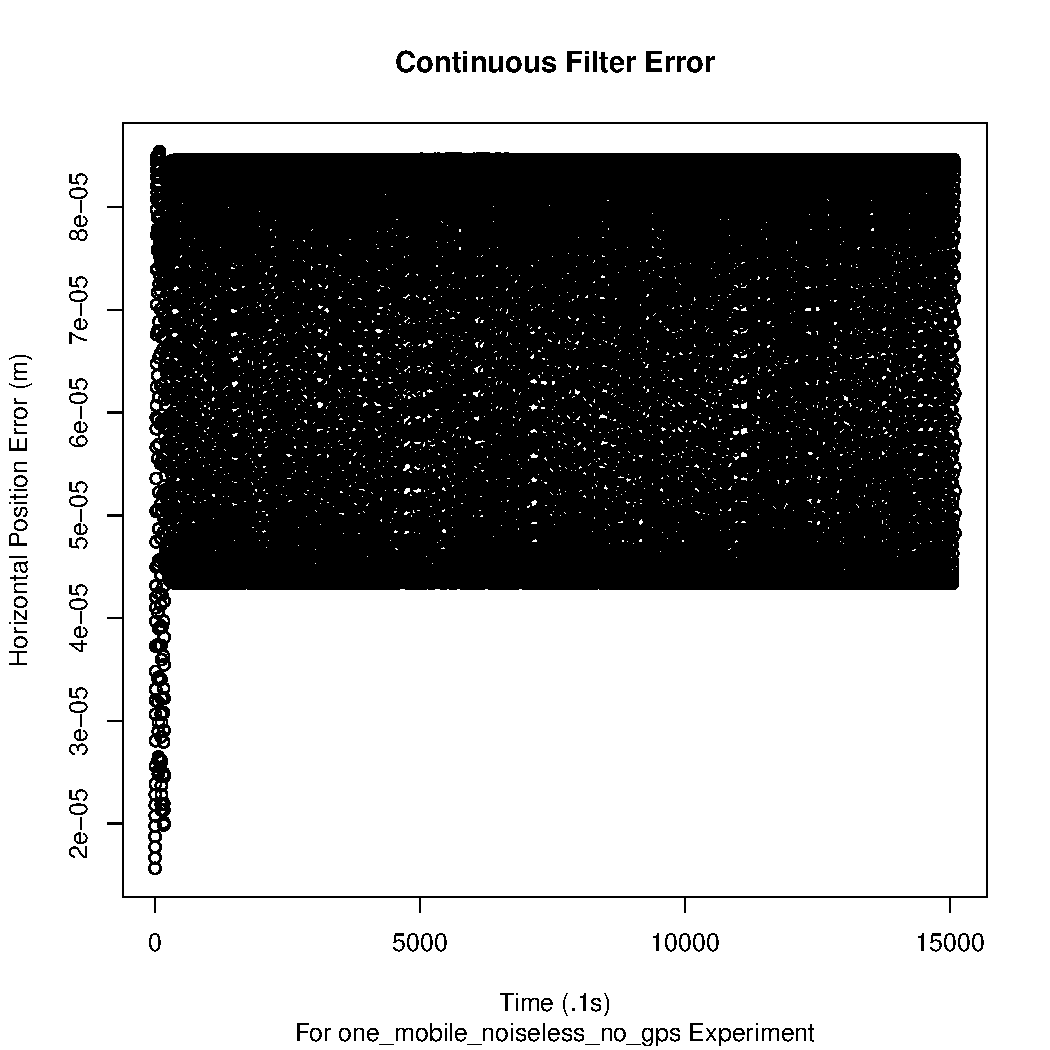
\includegraphics[width=\textwidth, keepaspectratio]{one_mobile_noiseless_no_gps_continuous_error}
\caption{Error of \gls{con_filter} of Mobile Robot with Noiseless Odometry Over Time}
\label{fig:one_mobile_noiseless_no_gps_continuous_error}
\end{figure}

From \autoref{tab:one_mobile_noiseless_no_gps_continuous_summary} we see that the maximum horizontal distance error is .116m with a mean error of .029m. Our robot has a radius of 0.2m, so our position estimate was always located within the radius of the robot. In the real world this error would be virtually undetectable. We also see that our maximum yaw error is .527 radians, which is not insignificant, however our mean error is -0.002 radians with a standard deviation of 0.110, which is very good. \autoref{fig:one_mobile_noiseless_no_gps_continuous_error} shows that our horizontal distance error is much more varied than in the stationary robot simulation, but this is still completely with the bounds of real-world perfection for localization.

\section{Noisy Individual Operation}
As shown in \autoref{sec:Control Group}, our simulation in a noiseless environment functions perfectly. This shows the accuracy of the \gls{kf} for localization and proves the functionality of our system. Now we should the same statistics for a stationary and mobile individual robot, but with the noise model implemented that was described in \autoref{sec:noise_model}.

\subsection{Stationary Robot}

% Table created by stargazer v.5.2 by Marek Hlavac, Harvard University. E-mail: hlavac at fas.harvard.edu
% Date and time: Tue, Aug 16, 2016 - 01:59:06 PM
\begin{table}[h] \centering 
  \caption{Continuous Filter Estimate for one-stationary Experiment} 
  \label{tab:one_stationary_continuous_summary} 
\begin{tabular}{@{\extracolsep{5pt}}lccccc} 
\\[-1.8ex]\hline 
\hline \\[-1.8ex] 
Statistic & \multicolumn{1}{c}{N} & \multicolumn{1}{c}{Mean} & \multicolumn{1}{c}{St. Dev.} & \multicolumn{1}{c}{Min} & \multicolumn{1}{c}{Max} \\ 
\hline \\[-1.8ex] 
x\_position & 458 & \num{0.0003} & \num{0.0001} & \num{0.00001} & \num{0.001} \\ 
y\_position & 458 & \num{0.00000003} & \num{0.00000003} & $-$0.000 & \num{0.0000001} \\ 
yaw & 458 & \num{0.0002} & \num{0.0001} & $-$0.00001 & \num{0.0004} \\ 
x\_variance & 458 & \num{1.536} & \num{0.839} & \num{0.076} & \num{2.993} \\ 
y\_variance & 458 & \num{1.536} & \num{0.839} & \num{0.076} & \num{2.993} \\ 
yaw\_variance & 458 & \num{1.841} & \num{1.006} & \num{0.091} & \num{3.588} \\ 
yaw\_error & 458 & \num{0.0001} & \num{0.00002} & \num{0.0001} & \num{0.0001} \\ 
x\_error & 458 & \num{0.000004} & \num{0.000001} & \num{0.000001} & \num{0.00001} \\ 
y\_error & 458 & \num{0.00000002} & \num{0.00000002} & \num{0.000} & \num{0.0000001} \\ 
horizontal\_error & 458 & \num{0.000004} & \num{0.000001} & \num{0.000001} & \num{0.00001} \\ 
\hline \\[-1.8ex] 
\end{tabular} 
\end{table} 


\begin{figure}
\centering
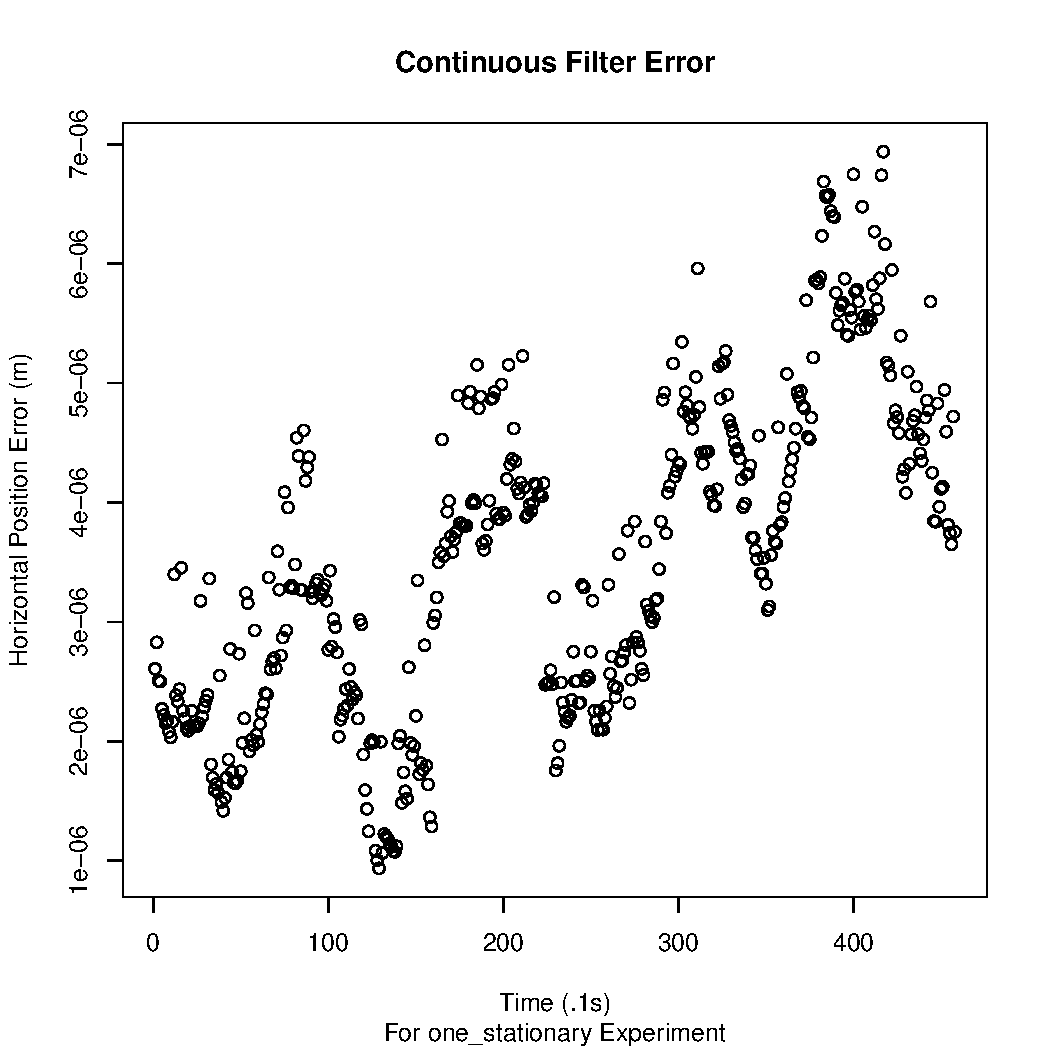
\includegraphics[width=\textwidth, keepaspectratio]{one_stationary_continuous_error}
\caption{Error of \gls{con_filter} of Stationary Robot with Noisy Odometry Over Time}
\label{fig:one_stationary_noisy_continuous_error}
\end{figure}

Comparing \autoref{tab:one_stationary_continuous_summary} to \autoref{tab:one_stationary_noiseless_no_gps_continuous_summary}, it is difficult to see a difference between the accuracy of the filter in the noisy vs. noiseless environment. However examining \autoref{fig:one_stationary_noisy_continuous_error} vs. \autoref{fig:one_stationary_noiseless_continuous_error}, it is clear the the addition of noise has affected the error of the filter. But this error is still so small that the filter is performing with what is realistically perfection. This is as we expect, because a stationary robot should have virtually no error. We can see this by looking at the noise model in \autoref{tab:sample_motion_model_odometry}. When the difference between $\bar{x}_{t-1}$ and $\bar{x}_t$ is almost 0, the standard deviations of our noise will also be almost 0, and this means there will be virtually no noise in the readings.


% Table created by stargazer v.5.2 by Marek Hlavac, Harvard University. E-mail: hlavac at fas.harvard.edu
% Date and time: Tue, Aug 09, 2016 - 09:46:29 AM
\begin{table}[h] \centering 
  \caption{Discrete Filter Estimate for one-stationary Experiment} 
  \label{tab:one_stationary_discrete_summary} 
\begin{tabular}{@{\extracolsep{5pt}}lccccc} 
\\[-1.8ex]\hline 
\hline \\[-1.8ex] 
Statistic & \multicolumn{1}{c}{N} & \multicolumn{1}{c}{Mean} & \multicolumn{1}{c}{St. Dev.} & \multicolumn{1}{c}{Min} & \multicolumn{1}{c}{Max} \\ 
\hline \\[-1.8ex] 
x\_position & 44,011 & 0.071 & 1.247 & $-$5.421 & 5.237 \\ 
y\_position & 44,011 & 0.022 & 1.112 & $-$3.544 & 4.152 \\ 
yaw & 44,011 & 0.015 & 0.009 & $-$0.005 & 0.030 \\ 
x\_error & 44,011 & $-$0.050 & 1.247 & $-$5.219 & 5.427 \\ 
y\_error & 44,011 & $-$0.022 & 1.112 & $-$4.152 & 3.544 \\ 
horizontal\_error & 44,011 & 1.335 & 1.007 & 0.002 & 5.529 \\ 
yaw\_error & 44,011 & 0.00004 & 0.0002 & $-$0.0001 & 0.005 \\ 
\hline \\[-1.8ex] 
\end{tabular} 
\end{table} 


\begin{figure}
\centering
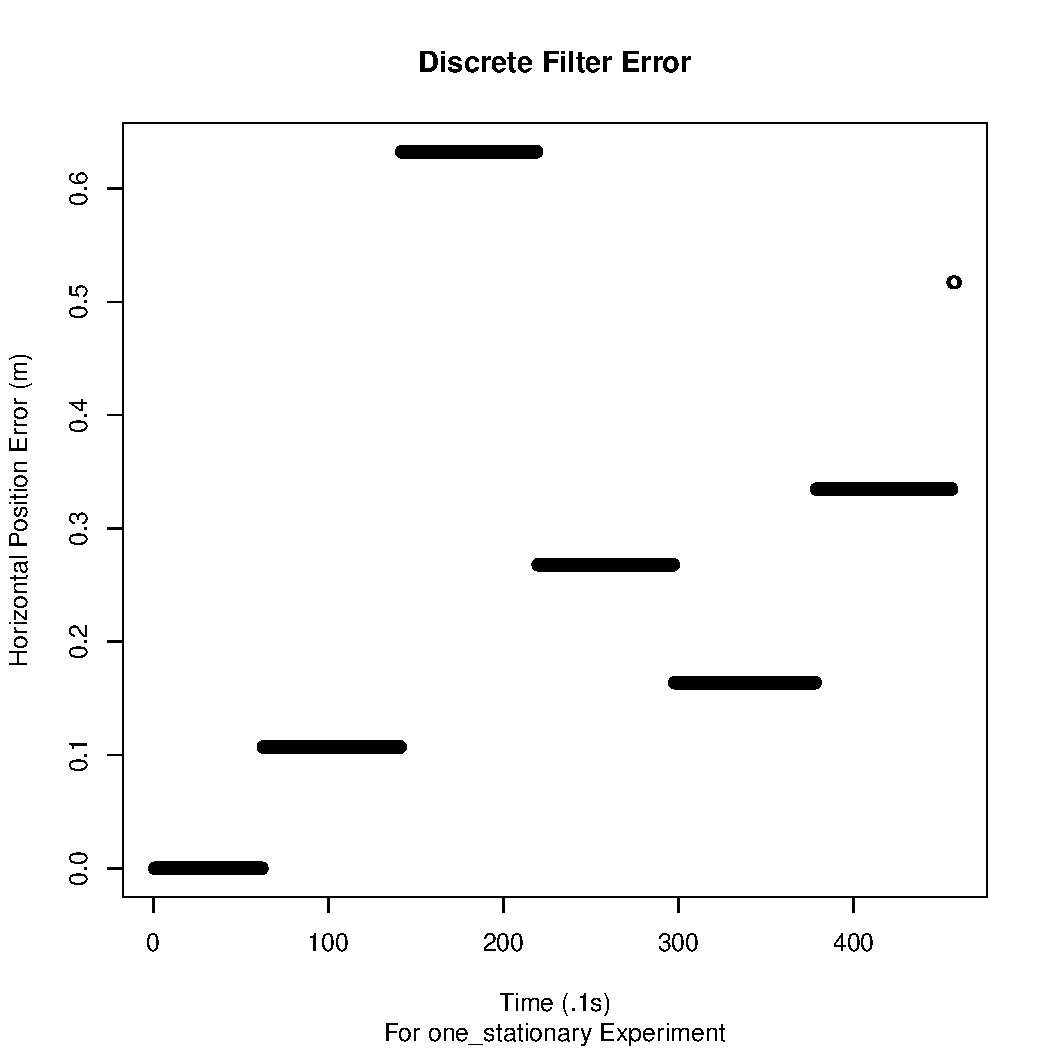
\includegraphics[width=\textwidth, keepaspectratio]{one_stationary_discrete_error}
\caption{Error of \gls{disc_filter} of Stationary Robot with Noisy Odometry Over Time}
\label{fig:one_stationary_noisy_dicrete_error}
\end{figure}

\subsection{Mobile Robot} \label{sec:Mobile Robot}

% Table created by stargazer v.5.2 by Marek Hlavac, Harvard University. E-mail: hlavac at fas.harvard.edu
% Date and time: Tue, Aug 09, 2016 - 09:46:14 AM
\begin{table}[h] \centering 
  \caption{Continuous Filter Estimate for one-mobile Experiment} 
  \label{tab:one_mobile_continuous_summary} 
\begin{tabular}{@{\extracolsep{5pt}}lccccc} 
\\[-1.8ex]\hline 
\hline \\[-1.8ex] 
Statistic & \multicolumn{1}{c}{N} & \multicolumn{1}{c}{Mean} & \multicolumn{1}{c}{St. Dev.} & \multicolumn{1}{c}{Min} & \multicolumn{1}{c}{Max} \\ 
\hline \\[-1.8ex] 
x\_position & 43,684 & 2.536 & 3.005 & $-$3.761 & 10.251 \\ 
y\_position & 43,684 & $-$2.040 & 5.072 & $-$15.305 & 10.223 \\ 
yaw & 43,684 & $-$0.011 & 1.809 & $-$3.142 & 3.142 \\ 
yaw\_error & 43,684 & $-$0.012 & 1.583 & $-$3.142 & 3.141 \\ 
x\_error & 43,684 & $-$2.757 & 6.071 & $-$22.602 & 6.839 \\ 
y\_error & 43,684 & 6.219 & 6.599 & $-$9.166 & 20.619 \\ 
horizontal\_error & 43,684 & 9.718 & 5.677 & 0.028 & 22.651 \\ 
\hline \\[-1.8ex] 
\end{tabular} 
\end{table} 


\begin{figure}
\centering
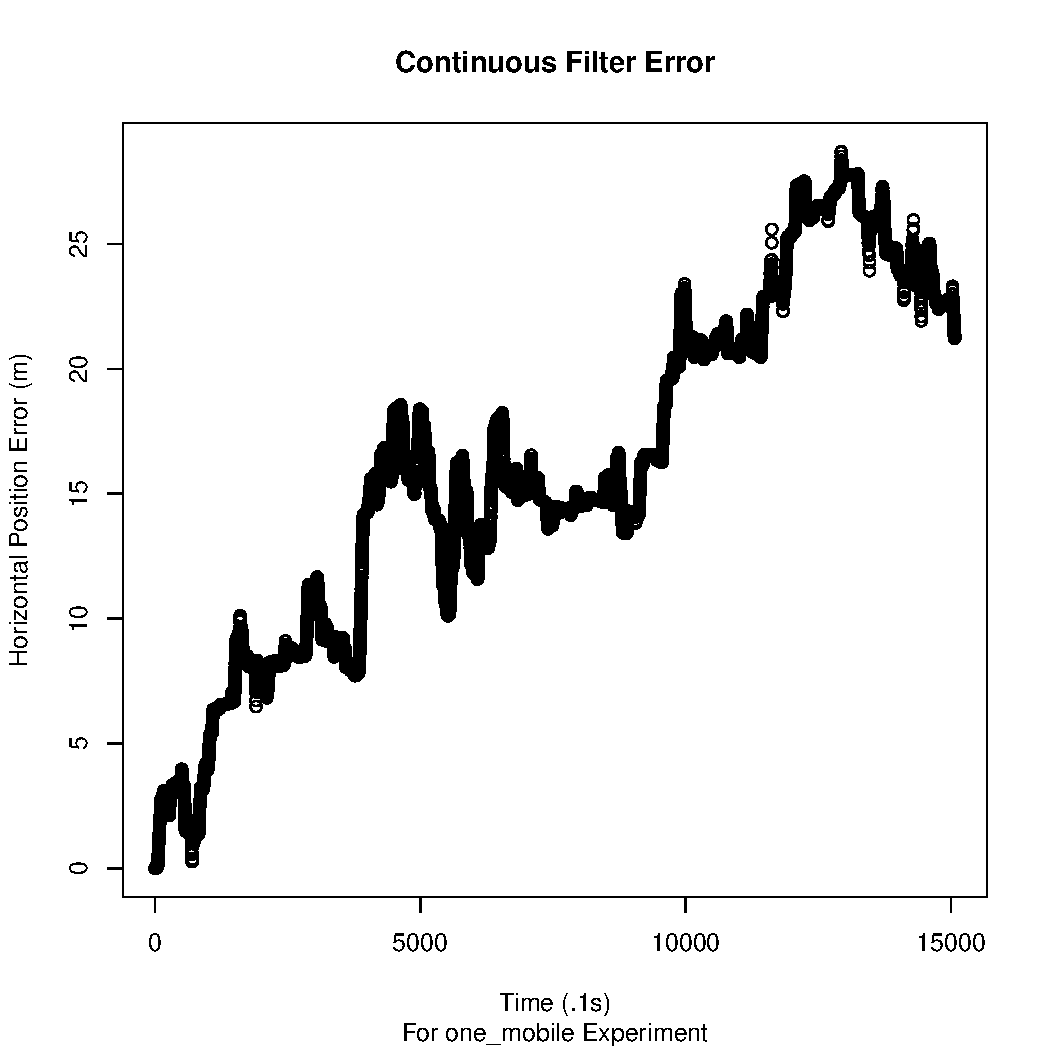
\includegraphics[width=\textwidth, keepaspectratio]{one_mobile_continuous_error}
\caption{Error of \gls{con_filter} of Mobile Robot with Noisy Odometry Over Time}
\label{fig:one_mobile_noisy_continuous_error}
\end{figure}

For the mobile robot, we see the effects of our noise model. The robot accumulates up to a maximum 30 meters of horizontal position error over its almost 30 minutes of operation. We also see a great increase in the yaw error, with a mean that is still close to 0 but a standard deviation of almost 2 radians.

This test of the mobile robot shows that our noise model is working as desired, and giving us a realistic model of odometry drift that a robot might see.


% Table created by stargazer v.5.2 by Marek Hlavac, Harvard University. E-mail: hlavac at fas.harvard.edu
% Date and time: Mon, Aug 15, 2016 - 10:02:13 PM
\begin{table}[htbp] \centering 
  \caption{Discrete Filter Location Estimate Error Summary for One Mobile Robot with Noisy Odometry and GPS} 
  \label{tab:one_mobile_discrete_summary} 
\begin{tabular}{@{\extracolsep{5pt}}lccccc} 
\\[-1.8ex]\hline 
\hline \\[-1.8ex] 
Statistic & \multicolumn{1}{c}{N} & \multicolumn{1}{c}{Mean} & \multicolumn{1}{c}{St. Dev.} & \multicolumn{1}{c}{Min} & \multicolumn{1}{c}{Max} \\ 
\hline \\[-1.8ex] 
x\_position (m) & 15,076 & \num{-0.868} & \num{3.504} & \num{-8.419} & \num{7.784} \\ 
y\_position (m) & 15,076 & \num{1.198} & \num{1.877} & \num{-3.695} & \num{7.539} \\ 
yaw (rad) & 15,076 & \num{-0.103} & \num{1.706} & \num{-3.141} & \num{3.141} \\ 
%%x\_variance & 15,076 & \num{1.483} & \num{0.261} & \num{0.071} & \num{4.915} \\ 
%%y\_variance & 15,076 & \num{1.458} & \num{0.215} & \num{0.071} & \num{4.559} \\ 
%%yaw\_variance & 15,076 & \num{0.409} & \num{0.206} & \num{0.085} & \num{2.231} \\ 
x\_error (m) & 15,076 & \num{-0.148} & \num{1.186} & \num{-5.424} & \num{4.077} \\ 
y\_error (m) & 15,076 & \num{0.189} & \num{1.201} & \num{-4.184} & \num{5.594} \\ 
yaw\_error (rad) & 15,076 & \num{-0.225} & \num{1.606} & \num{-3.141} & \num{3.140} \\ 
position\_error (m) & 15,076 & \num{1.366} & \num{1.019} & \num{0.00001} & \num{6.037} \\ 
\hline \\[-1.8ex] 
\end{tabular} 
\end{table} 


\begin{figure}
\centering
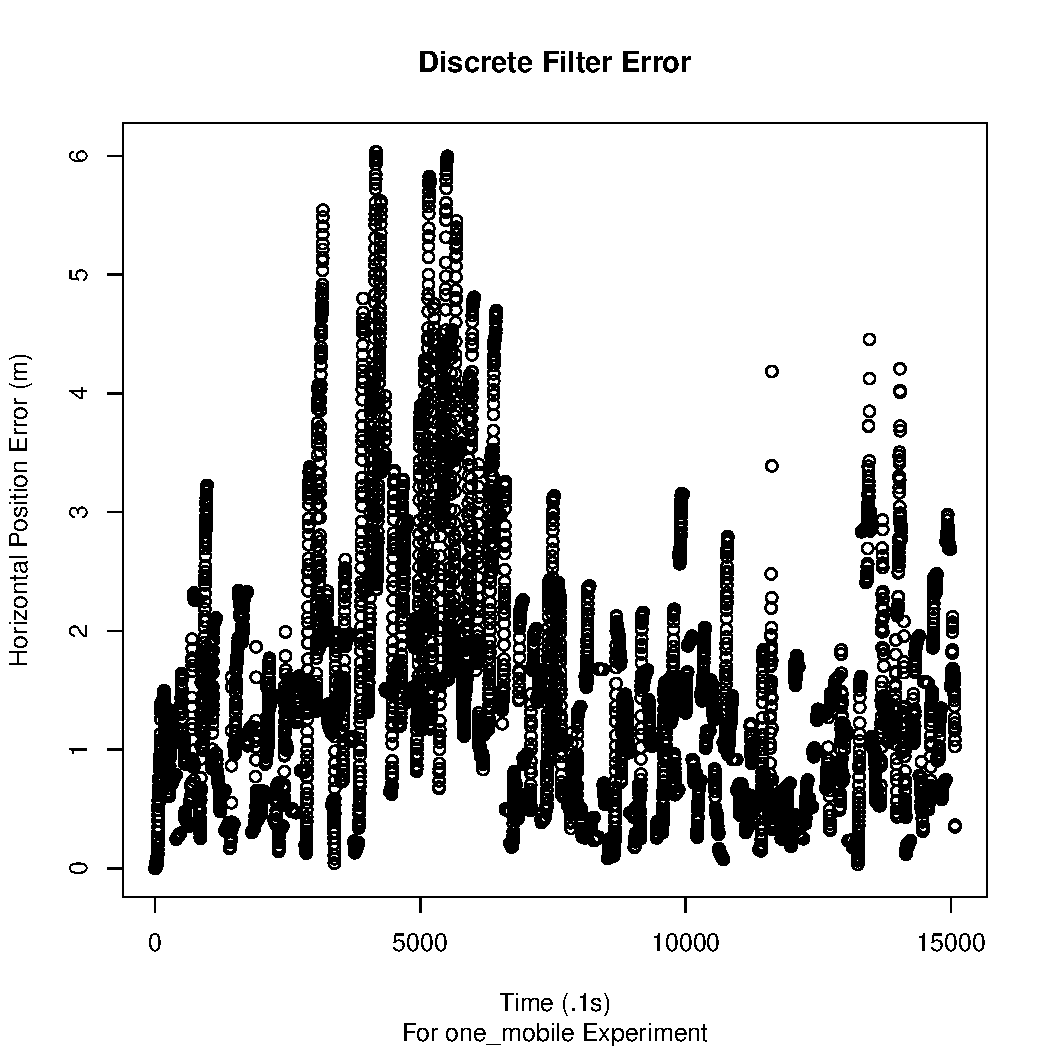
\includegraphics[width=\textwidth, keepaspectratio]{one_mobile_discrete_error}
\caption{Error of \gls{disc_filter} of Mobile Robot with Noisy Odometry Over Time}
\label{fig:one_mobile_discrete_error}
\end{figure}

For the single mobile robot we also examine the error in the discrete filter, shown in \autoref{tab:one_mobile_discrete_summary} and \autoref{fig:one_mobile_discrete_error}. For a single robot experiment, this filter receives only the robot's odometry and GPS as inputs. This acts as our control experiment for the discrete filter, we expect to see increased accuracy with the addition of the external pose readings. We see that the addition of the GPS greatly increases the accuracy of the filter.

\section{Noisy Group Operation}

% Table created by stargazer v.5.2 by Marek Hlavac, Harvard University. E-mail: hlavac at fas.harvard.edu
% Date and time: Mon, Aug 15, 2016 - 04:28:03 PM
\begin{table}[h] \centering 
  \caption{Discrete Filter Estimate for two-stationary Experiment} 
  \label{tab:two_stationary_discrete_summary} 
\begin{tabular}{@{\extracolsep{5pt}}lccccc} 
\\[-1.8ex]\hline 
\hline \\[-1.8ex] 
Statistic & \multicolumn{1}{c}{N} & \multicolumn{1}{c}{Mean} & \multicolumn{1}{c}{St. Dev.} & \multicolumn{1}{c}{Min} & \multicolumn{1}{c}{Max} \\ 
\hline \\[-1.8ex] 
x\_position & 1,007 & 0.522 & 1.027 & $-$0.896 & 1.970 \\ 
y\_position & 1,007 & 0.522 & 0.408 & $-$0.000 & 1.264 \\ 
yaw & 1,007 & 0.0002 & 0.0001 & $-$0.000 & 0.0005 \\ 
x\_variance & 1,007 & 0.522 & 0.590 & 0.002 & 1.652 \\ 
y\_variance & 1,007 & 0.522 & 0.590 & 0.002 & 1.652 \\ 
yaw\_variance & 1,007 & 0.379 & 0.171 & 0.088 & 0.689 \\ 
x\_error & 1,007 & 0.471 & 0.283 & 0.00001 & 0.926 \\ 
y\_error & 1,007 & $-$0.522 & 0.408 & $-$1.264 & 0.000 \\ 
horizontal\_error & 1,007 & 0.723 & 0.467 & 0.00001 & 1.567 \\ 
yaw\_error & 1,007 & 0.00005 & 0.00004 & $-$0.00004 & 0.0002 \\ 
\hline \\[-1.8ex] 
\end{tabular} 
\end{table} 


\begin{figure}
\centering
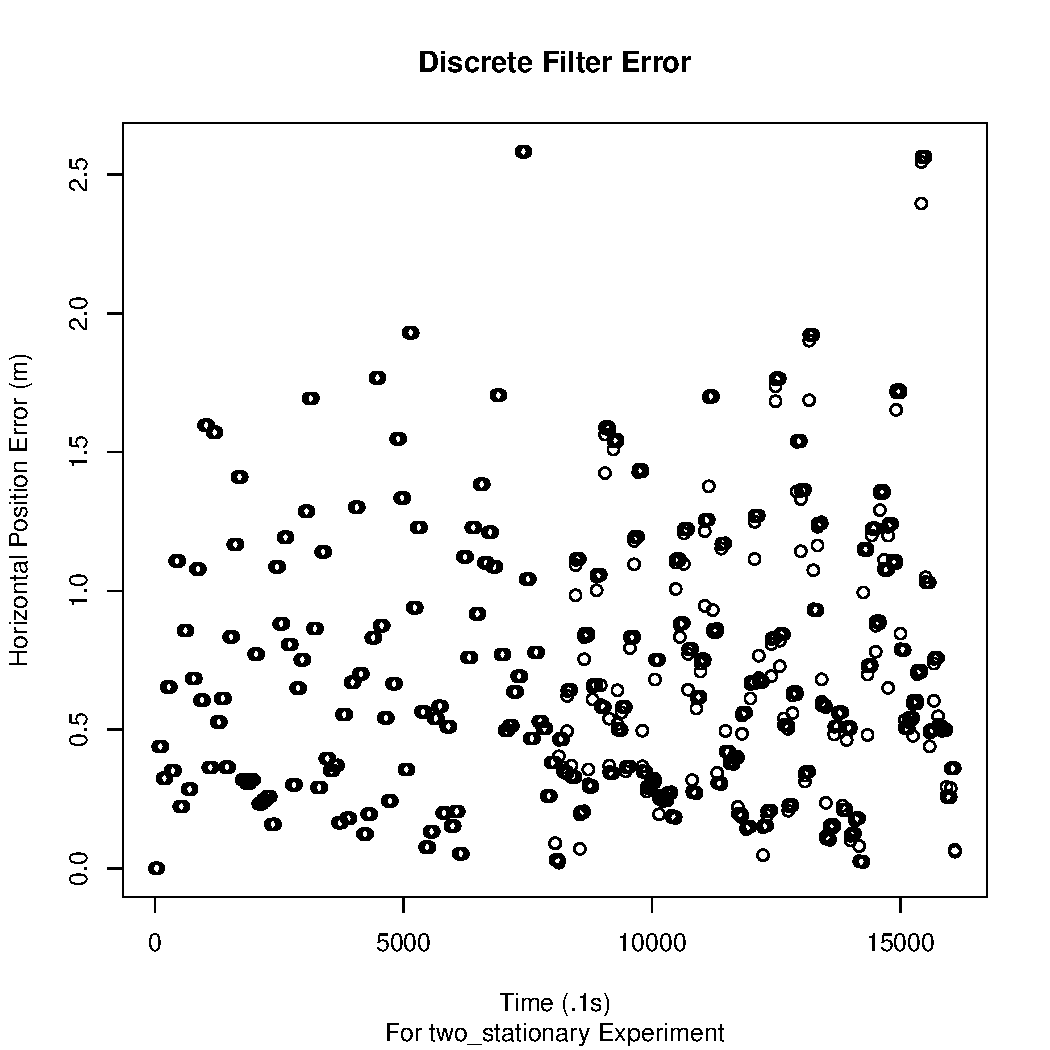
\includegraphics[width=\textwidth, keepaspectratio]{two_stationary_discrete_error}
\caption{Error of \gls{disc_filter} for Mobile Robots with Noisy Odometry Over Time}
\label{fig:two_stationary_discrete_error}
\end{figure}


% Table created by stargazer v.5.2 by Marek Hlavac, Harvard University. E-mail: hlavac at fas.harvard.edu
% Date and time: Mon, Aug 15, 2016 - 10:04:41 PM
\begin{table}[h] \centering 
  \caption{Discrete Filter Estimate for two-mobile Experiment} 
  \label{tab:two_mobile_discrete_summary} 
\begin{tabular}{@{\extracolsep{5pt}}lccccc} 
\\[-1.8ex]\hline 
\hline \\[-1.8ex] 
Statistic & \multicolumn{1}{c}{N} & \multicolumn{1}{c}{Mean} & \multicolumn{1}{c}{St. Dev.} & \multicolumn{1}{c}{Min} & \multicolumn{1}{c}{Max} \\ 
\hline \\[-1.8ex] 
x\_position & 30,750 & $-$0.164 & 1.008 & $-$3.112 & 4.145 \\ 
y\_position & 30,750 & $-$0.813 & 1.182 & $-$5.443 & 3.951 \\ 
yaw & 30,750 & 0.084 & 0.398 & $-$3.141 & 3.058 \\ 
x\_variance & 30,750 & 1.360 & 0.355 & 0.0002 & 2.569 \\ 
y\_variance & 30,750 & 1.362 & 0.360 & 0.0002 & 4.066 \\ 
yaw\_variance & 30,750 & 0.392 & 0.177 & 0.090 & 2.186 \\ 
x\_error & 30,750 & $-$0.070 & 0.857 & $-$3.368 & 2.743 \\ 
y\_error & 30,750 & $-$0.011 & 0.781 & $-$4.071 & 2.714 \\ 
horizontal\_error & 30,750 & 0.954 & 0.663 & 0.00002 & 4.213 \\ 
yaw\_error & 30,750 & $-$0.011 & 0.389 & $-$3.141 & 3.141 \\ 
\hline \\[-1.8ex] 
\end{tabular} 
\end{table} 


\begin{figure}
\centering
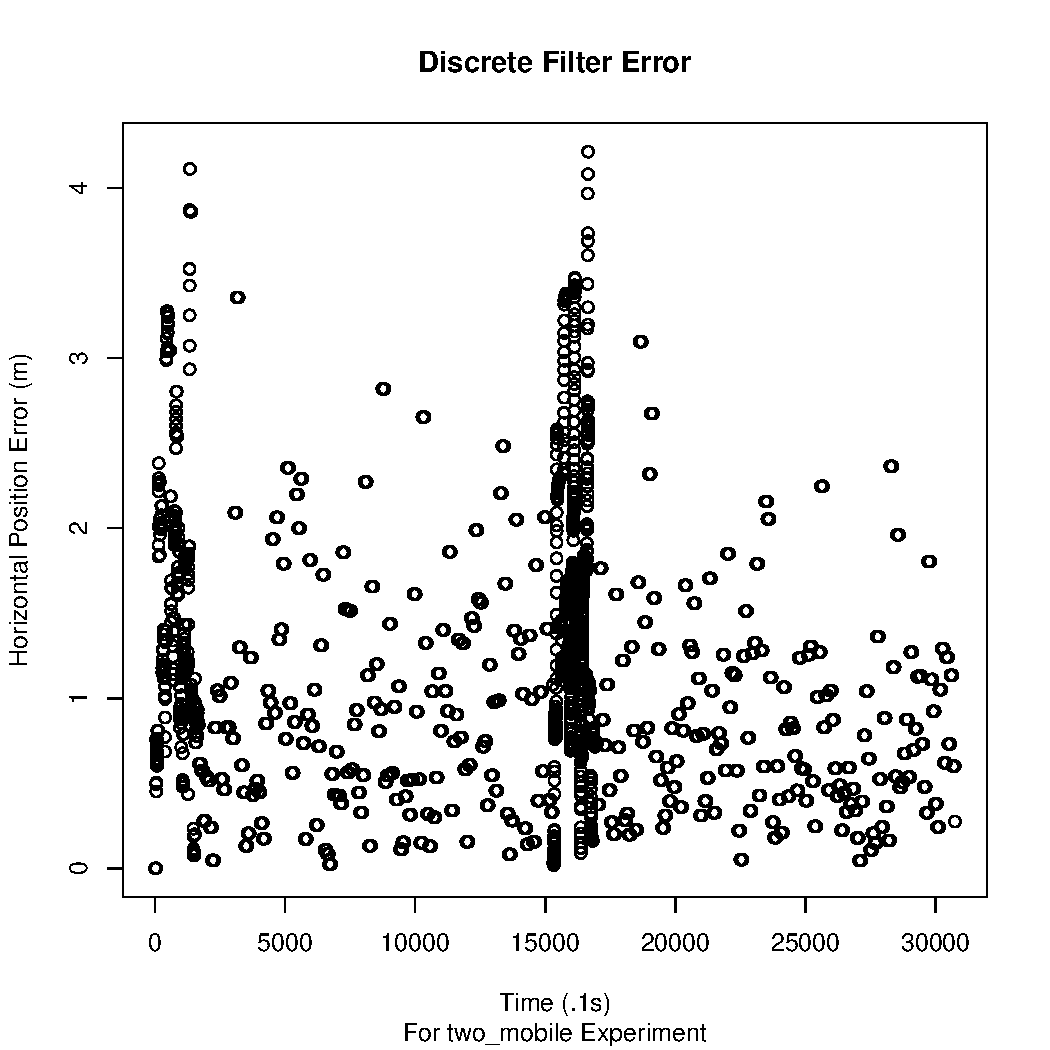
\includegraphics[width=\textwidth, keepaspectratio]{two_mobile_discrete_error}
\caption{Error of \gls{disc_filter} for Mobile Robots with Noisy Odometry Over Time}
\label{fig:two_mobile_discrete_error}
\end{figure}

Finally, we operate in a group. For these experiments, we are not concerned with information about the \gls{con_filter}, because we have already proved its functionality in the preceding sections. Because the \gls{con_filter}'s only input is the robot's odometry, no changes will be seen when operating individually vs. in a group.

What does change is the \gls{disc_filter}. Operating in a group means the \gls{disc_filter} now receives external pose measurements from other robots. \autoref{tab:two_mobile_discrete_summary} and \autoref{fig:two_mobile_discrete_error} show the error of the discrete filter with two robots operating in the same environment.

\section{Increased Robot Density}

% Table created by stargazer v.5.2 by Marek Hlavac, Harvard University. E-mail: hlavac at fas.harvard.edu
% Date and time: Tue, Aug 09, 2016 - 09:47:07 AM
\begin{table}[h] \centering 
  \caption{Discrete Filter Estimate for two-mobile-restricted Experiment} 
  \label{tab:two_mobile_restricted_discrete_summary} 
\begin{tabular}{@{\extracolsep{5pt}}lccccc} 
\\[-1.8ex]\hline 
\hline \\[-1.8ex] 
Statistic & \multicolumn{1}{c}{N} & \multicolumn{1}{c}{Mean} & \multicolumn{1}{c}{St. Dev.} & \multicolumn{1}{c}{Min} & \multicolumn{1}{c}{Max} \\ 
\hline \\[-1.8ex] 
x\_position & 93,797 & $-$7.461 & 11.437 & $-$59.781 & 15.809 \\ 
y\_position & 93,797 & 0.756 & 3.941 & $-$27.260 & 16.565 \\ 
yaw & 93,797 & 0.028 & 1.840 & $-$3.141 & 3.141 \\ 
x\_error & 93,797 & 0.202 & 3.317 & $-$15.285 & 60.469 \\ 
y\_error & 93,797 & 0.109 & 2.078 & $-$16.028 & 28.646 \\ 
horizontal\_error & 93,797 & 1.989 & 3.380 & 0.001 & 65.610 \\ 
yaw\_error & 93,797 & 0.039 & 1.683 & $-$3.142 & 3.141 \\ 
\hline \\[-1.8ex] 
\end{tabular} 
\end{table} 


\begin{figure}
\centering
\includegraphics[width=\textwidth, keepaspectratio]{two_mobile_restricted_discrete_error}
\caption{Error of \gls{disc_filter} for Mobile Robots with Noisy Odometry Over Time}
\label{fig:two_mobile_restricted_discrete_error}
\end{figure}

%\section{Five Robot}
%
% Table created by stargazer v.5.2 by Marek Hlavac, Harvard University. E-mail: hlavac at fas.harvard.edu
% Date and time: Tue, Aug 09, 2016 - 09:46:05 AM
\begin{table}[h] \centering 
  \caption{Discrete Filter Estimate for five-mobile Experiment} 
  \label{tab:five_mobile_discrete_summary} 
\begin{tabular}{@{\extracolsep{5pt}}lccccc} 
\\[-1.8ex]\hline 
\hline \\[-1.8ex] 
Statistic & \multicolumn{1}{c}{N} & \multicolumn{1}{c}{Mean} & \multicolumn{1}{c}{St. Dev.} & \multicolumn{1}{c}{Min} & \multicolumn{1}{c}{Max} \\ 
\hline \\[-1.8ex] 
x\_position & 69,192 & 0.813 & 41.936 & $-$209.465 & 210.747 \\ 
y\_position & 69,192 & 9.634 & 40.915 & $-$192.420 & 173.376 \\ 
yaw & 69,192 & 0.066 & 1.758 & $-$3.141 & 3.141 \\ 
x\_error & 69,192 & $-$0.109 & 41.989 & $-$211.164 & 213.926 \\ 
y\_error & 69,192 & $-$9.833 & 40.885 & $-$174.640 & 193.392 \\ 
horizontal\_error & 69,192 & 45.689 & 37.998 & 0.005 & 221.287 \\ 
yaw\_error & 69,192 & 0.112 & 1.251 & $-$3.142 & 3.141 \\ 
\hline \\[-1.8ex] 
\end{tabular} 
\end{table} 

%
%\begin{figure}
%\centering
%\includegraphics[width=\textwidth, keepaspectratio]{five_mobile_discrete_error}
%\caption{Error of \gls{disc_filter} for Mobile Robots with Noisy Odometry Over Time}
%\label{fig:five_mobile_discrete_error}
%\end{figure}
%
%\input{autogenerated_tables/five_mobile_restricted_discrete_summary.tex}
%
%\begin{figure}
%\centering
%\includegraphics[width=\textwidth, keepaspectratio]{five_mobile_restricted_discrete_error}
%\caption{Error of \gls{disc_filter} for Mobile Robots with Noisy Odometry Over Time}
%\label{fig:five_mobile_restricted_discrete_error}
%\end{figure}

\end{document}